\begin{frame}
  \frametitle{Lecture d'une ligne par le simulateur}
  
  \begin{figure}[h!]
    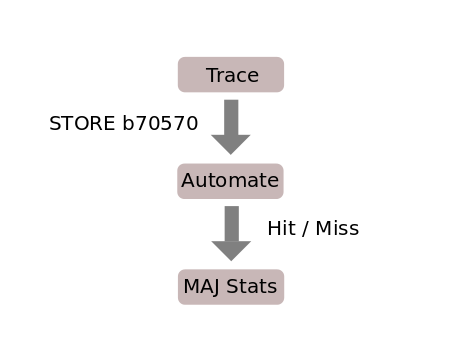
\includegraphics[width=0.75\textwidth]{images/cassis_deroulement.png}
  \end{figure}
  
\end{frame}

\begin{frame}[fragile]
  \frametitle{Données d'entrée de \emph{Cassis}}
  
%  \begin{figure}[h!]
%    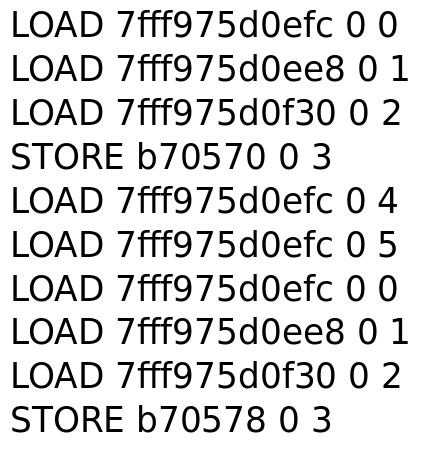
\includegraphics[width=.4\textwidth]{images/traces.png}
%  \end{figure}
  
  \begin{itemize}
    \item{Fichier de description d'architecture}
    \item{Trace d'exécution}
  \end{itemize}
  
\begin{verbatim}
LOAD 7fff975d0efc 0 0
LOAD 7fff975d0ee8 0 1
LOAD 7fff975d0f30 0 2
STORE b70570 0 3
LOAD 7fff975d0efc 0 4
LOAD 7fff975d0efc 0 5
LOAD 7fff975d0efc 0 0
LOAD 7fff975d0ee8 0 1
LOAD 7fff975d0f30 0 2
STORE b70578 0 3
...
\end{verbatim}

\end{frame}

\begin{frame}[fragile]
  \frametitle{Statistiques}
  
  \begin{block}{Statistiques basiques}
    \begin{itemize}
    \item{Hit}
    \item{Miss}
    \item{Write-back}
    \end{itemize}
  \end{block}
  
  \begin{columns}[T]
    \begin{column}{.5\textwidth}
      \begin{figure}[h!]
	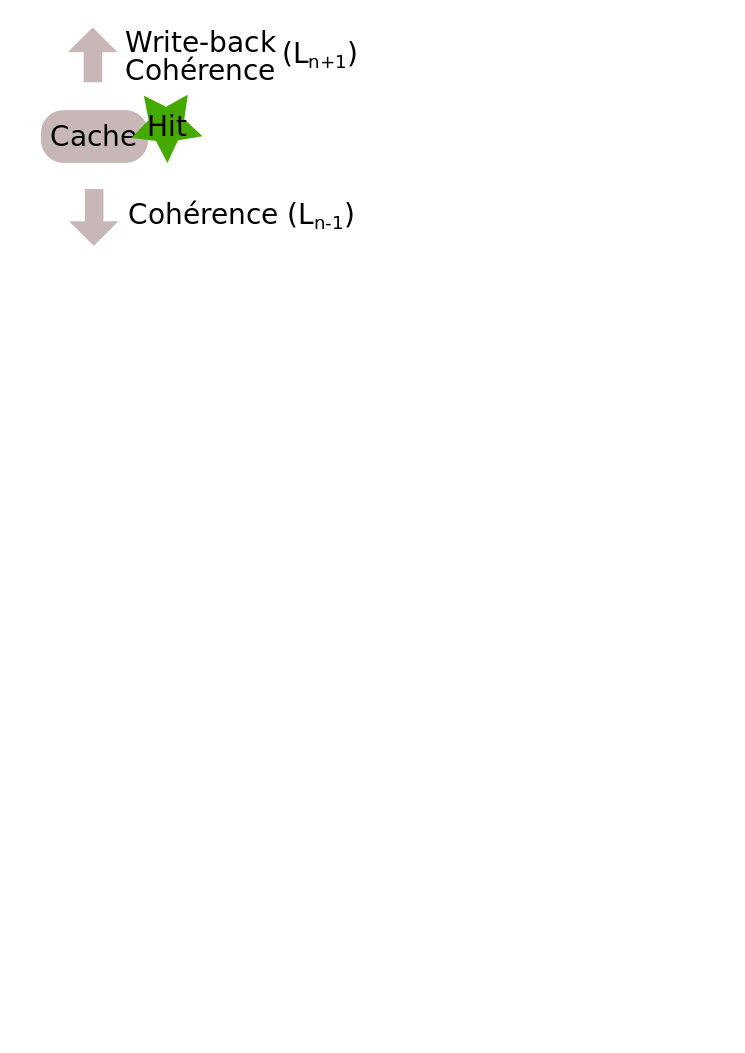
\includegraphics[scale=.4]{images/evictions.png}
      \end{figure}
    \end{column}
    \begin{column}{.5\textwidth}
      \bigskip
      \begin{block}{Types d'évictions}
	\begin{itemize}
	\item{Cohérence}
        \item{Capacité}
        \item{Type de cache         }
	\end{itemize}
      \end{block}
    \end{column}
  \end{columns}
\end{frame}

\begin{frame}[fragile]
  \frametitle{Statistiques}
  
  \begin{block}{Statistiques globales}
    \begin{itemize}
    \item{Broadcast cohérence}
    \item{Broadcast de snooping}
    \end{itemize}
  \end{block}
  
  \begin{columns}[T]
    \begin{column}{.5\textwidth}
      \begin{figure}[h!]
	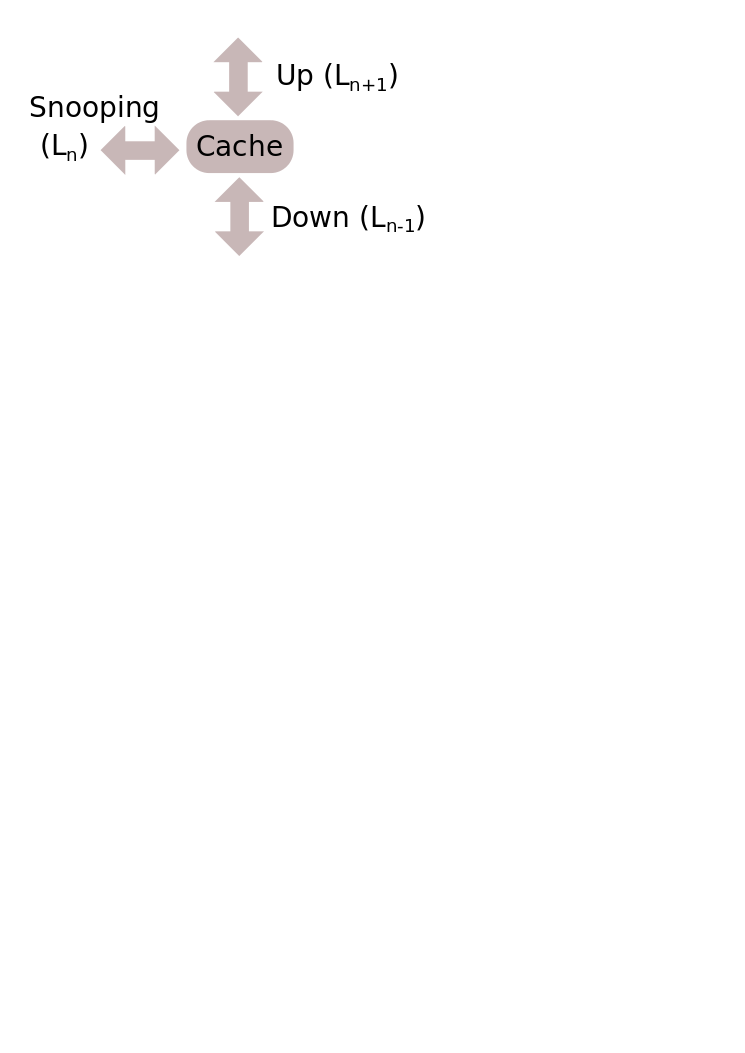
\includegraphics[scale=.4]{images/misses.png}
      \end{figure}
    \end{column}
    \begin{column}{.5\textwidth}
      \bigskip
      \begin{block}{Types de misses}
	\begin{itemize}
	\item{Snooping}
        \item{Cache de niveau supérieur}
        \item{Cache de niveau inférieur}
	\end{itemize}
      \end{block}
    \end{column}
  \end{columns}
\end{frame}
